\chapter{Introducción específica} % Main chapter title

\label{Chapter2}

%----------------------------------------------------------------------------------------
%	2.1 ENFOQUE DEL PROBLEMA
%----------------------------------------------------------------------------------------
ESCRIBIR PARRAFO INTRODUCTORIO

\section{Enfoque del problema}
\label{sec:Enfoque del problema}

El presente trabajo se estructura en torno a tres etapas principales, las cuales se 
encuentran ilustradas en la figura \ref{fig:Etapas de trabajo}.


\begin{figure}[ht]
	\centering
	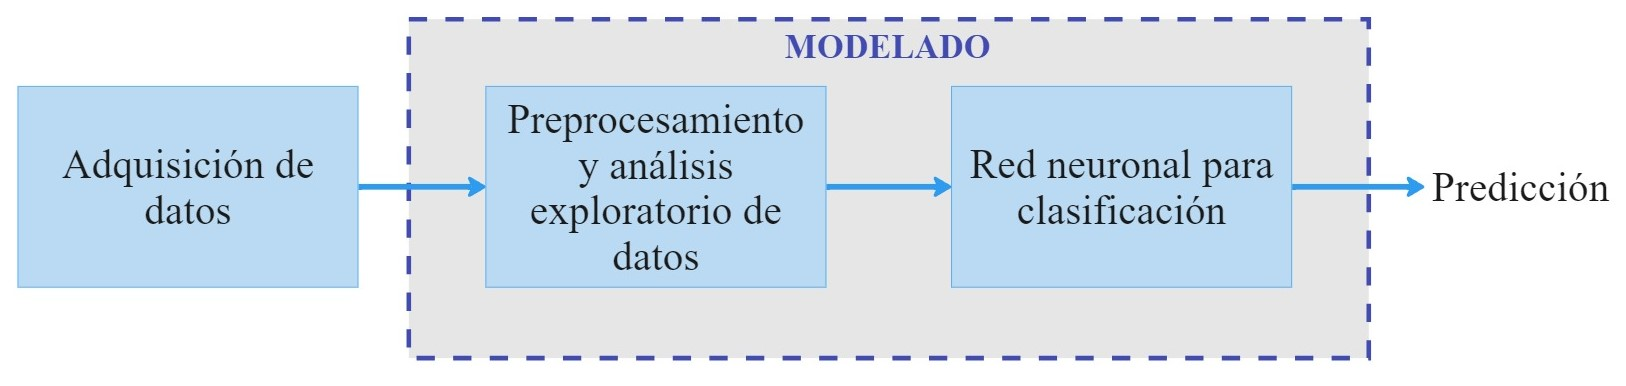
\includegraphics[width=\textwidth]{./Figures/Etapas de trabajo.jpg}
	\caption{Representación esquemática de las etapas del trabajo.}\label{fig:Etapas de trabajo}
\end{figure}

Para comenzar, se llevó a cabo la adquisición de datos. 
Esta etapa fue realizada en colaboración con el servicio de cardiología del Hospital Alemán. 
Para ello, se recopiló información proveniente de presurometrías realizadas a pacientes 
hipertensos a partir del año 2013. Además, se efectuó un análisis exhaustivo de la historia 
clínica de cada paciente con el objetivo de identificar la ocurrencia de eventos cardiovasculares 
adversos mayores. De esta manera, se logró completar el \textit{dataset} con la variable a predecir (MACE) 
para cada paciente. Asimismo, se enriqueció el conjunto de datos con información clínica adicional 
con el fin de contar con variables explicativas más amplias para abordar el problema de investigación.

A continuación, se efectuó una etapa de preprocesamiento. En primer lugar, se procedió a realizar 
una limpieza de los datos con el propósito de seleccionar las variables más representativas del 
problema. Este proceso de selección permitió eliminar datos redundantes, ruidosos o de poca 
utilidad para el análisis posterior. También, se realizó un análisis exploratorio de datos 
para comprender de manera más profunda las características y patrones presentes en el \textit{dataset}. 
Esto proporcionó una visión más completa y significativa del conjunto de datos, permitiendo 
así una mejor comprensión de la naturaleza del problema y orientando la toma de decisiones 
posteriores en el desarrollo de este trabajo.

Por último, se procedió al diseñó y entrenamiento de dos modelos de clasificación utilizando 
redes neuronales. El primer modelo se construyó exclusivamente con los datos de presurometrías, 
mientras que el segundo modelo se enriqueció al incluir también los datos clínicos. El propósito 
de esta estrategia fue analizar y comparar el rendimiento de los dos modelos y evaluar si los 
datos de MAPA tienen un sustento suficiente para predecir la variable objetivo MACE. De esta 
manera, se buscó determinar si la inclusión de información clínica adicional contribuyó a 
mejorar las métricas de desempeño en la predicción de MACE, y si podría tener implicancias 
clínicas relevantes para el seguimiento de los pacientes.

%----------------------------------------------------------------------------------------
%	2.2 ALGORITMOS DE CLASIFICACION
%----------------------------------------------------------------------------------------
\section{Algoritmos de clasificación}
\label{sec:Algoritmos de clasificación}

En esta sección se presentan los fundamentos de los modelos de clasificación, junto con las 
estrategias utilizadas para abordar el desbalance de clases, con especial énfasis en la técnica SMOTE. 
Además, se exploran las métricas utilizadas para evaluar el desempeño de los modelos desarrollados.

%----------------------------------------------------------------------------------------
% 2.2.1 Fundamentos de los modelos de clasificación

\subsection{Fundamentos de los modelos de clasificación}
Un algoritmo de aprendizaje automático es una herramienta que permite resolver tareas  
que suelen ser complejas de abordar para los seres humanos. La principal ventaja del \emph{machine 
learning} (ML) es su capacidad de aprender de los datos y extraer información relevante de 
estos. Las tareas de ML se describen en términos de cómo deben procesar un ejemplo, que se 
compone de una colección de características cuantitativas o \emph{features} que se miden de un objeto 
o evento que se desea procesar. En general, se representa un ejemplo como un vector $ x\in\mathbb{R}^n $,
donde cada entrada $x_{i}$ del vector corresponde a una característica del objeto 
o evento en cuestión. De esta manera, el algoritmo de aprendizaje de máquina es capaz de 
analizar los datos y extraer patrones que permiten tomar decisiones o realizar predicciones 
precisas \citep{CITE:35}.

En el campo del aprendizaje automático, los modelos de clasificación desempeñan un papel fundamental 
\citep{CITE:32}. Estos modelos se encargan de asignar etiquetas discretas o categorías a ejemplos 
específicos según sus características \citep{CITE:33}. Dependiendo del enfoque utilizado durante el 
entrenamiento, los modelos pueden ser de dos tipos: supervisados o no supervisados \citep{CITE:35}.

En un modelo de clasificación no supervisado, las etiquetas no se proporcionan en el conjunto de 
datos de entrenamiento \citep{CITE:34}. En lugar de ello, el algoritmo busca patrones y estructuras 
en los datos sin la guía explícita de las etiquetas. Como resultado, el objetivo es agrupar las instancias en 
clases basadas en similitudes \citep{CITE:33}.

Por otro lado, en un modelo de clasificación supervisado se proporciona al algoritmo un \emph{dataset} de 
entrenamiento que incluye tanto las características de las instancias como las etiquetas correspondientes 
\citep{CITE:33}. El modelo utiliza esta información para aprender a asociar las \emph{features} con las 
etiquetas, lo que le permite clasificar nuevas instancias de manera precisa. Algunos ejemplos de algoritmos 
supervisados ampliamente utilizados son los árboles de decisión, las máquinas de vectores de soporte y 
las redes neuronales \citep{CITE:34}. En este trabajo en particular, se empleó un modelo de clasificación 
supervisado basado en redes neuronales con el propósito de predecir MACE. Es importante señalar que se trata
de una clasificación binaria puesto que la variable \emph{target} tiene dos posibles valores: ausencia ("0") o 
presencia ("1") de eventos cardiovasculares adversos mayores.

%----------------------------------------------------------------------------------------
% 2.2.2 Estrategias para tratar el desbalance de clases
\subsection{Estrategias para tratar el desbalance de clases}

Un conjunto de datos se considera desbalanceado cuando presenta una proporción significativamente mayor 
de observaciones pertenecientes a una clase en comparación con la otra. Este desequilibrio puede tener 
un impacto considerable en el rendimiento de los modelos de aprendizaje automático. En el caso específico 
de una red neuronal entrenada con un \emph{dataset} desbalanceado, es probable que encuentre dificultades 
para discriminar de manera adecuada entre las diferentes clases. En otras palabras, el desequilibrio de 
clases crea un sesgo en el cual el modelo tiende a predecir la clase mayoritaria, lo que dificulta la 
correcta clasificación de los ejemplos pertenecientes a la clase minoritaria \citep{CITE:36} \citep{CITE:37}. 

Abordar el desequilibrio se convierte en un desafío crucial en la tarea de modelado y actualmente existen 
dos enfoques principales. El primero consiste en asignar diferentes pesos a los ejemplos de entrenamiento, 
mientras que el segundo implica realizar un remuestreo del conjunto de datos original. Es posible crear 
un nuevo muestreo del \emph{dataset} efectuando un sobremuestreo de la clase minoritaria y/o un submuestreo 
de la clase mayoritaria. El submuestreo implica una reducción del número de instancias de la clase mayoritaria, 
lo cual puede resultar en la pérdida de información valiosa que sea representativa de la distribución de los 
datos. Por otra parte, el sobremuestreo suele implicar réplicas de ejemplos de la clase minoritaria, lo cual 
puede generar un sobreajuste. En concreto, el modelo concede predicciones muy precisas para el conjunto de 
entrenamiento pero no logra generalizar adecuadamente cuando se presentan nuevos datos \citep{CITE:37}. 

Para mitigar las desventajas mencionadas anteriormente, Nitesh Chawla \emph{et al.} \citep{CITE:37} 
introducen una nueva técnica que implica una forma especial 
de sobremuestrear la clase minoritaria. El algoritmo 
\emph{Synthetic Minority Over-sampling Technique} (SMOTE) implica la creación de muestras sintéticas de 
la clase minoritaria. Se expone una representación gráfica del algoritmo en la figura \ref{fig:SMOTE}. 
En primer lugar, el método escoge un ejemplo de la clase minoritaria al azar y encuentra a sus $k$ vecinos 
más cercanos. Luego, se selecciona uno de los $k$ vecinos más cercanos y se crea una conexión mediante 
un segmento de línea en el espacio de características con la muestra elegida al azar. Finalmente, se crea 
una instancia sintética en un punto aleatorio entre los dos ejemplos. Este procedimiento se repite para
todas las muestras minoritarias \citep{CITE:38}. 

\begin{figure}[h!]
	\centering
	\subcaptionbox{SMOTE comienza con un conjunto de ejemplos positivos (puntos verdes) y negativos (puntos azules).}%
  	[0.3\linewidth]{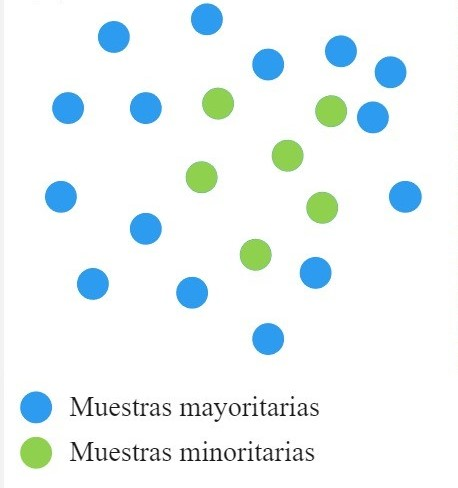
\includegraphics[height=5cm]{./Figures/SMOTE_a.jpg}}\label{fig:SMOTEa}
	\hspace{1em}
	\subcaptionbox{Se selecciona un ejemplo positivo (punto con borde negro) y sus $k$ vecinos más cercanos entre los positivos (puntos amarillos, con $k = 3$).}
	[0.3\linewidth]{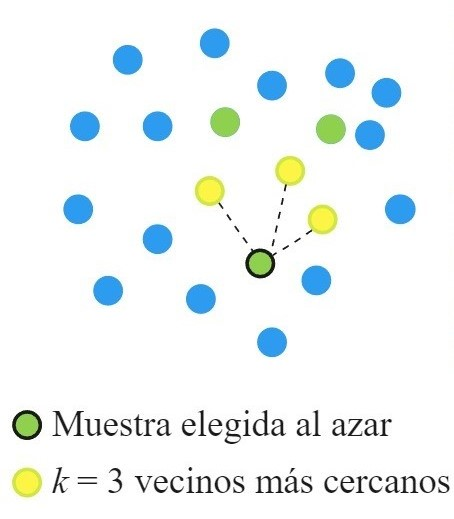
\includegraphics[height=5cm]{./Figures/SMOTE_b.jpg}}\label{fig:SMOTEb}
	\hspace{1em}
	\subcaptionbox{Para cada $k$ vecino más cercano se agrega un nuevo ejemplo sintético (puntos rojos) a lo largo de la línea recta que los conecta con el ejemplo positivo.}
	[0.3\linewidth]{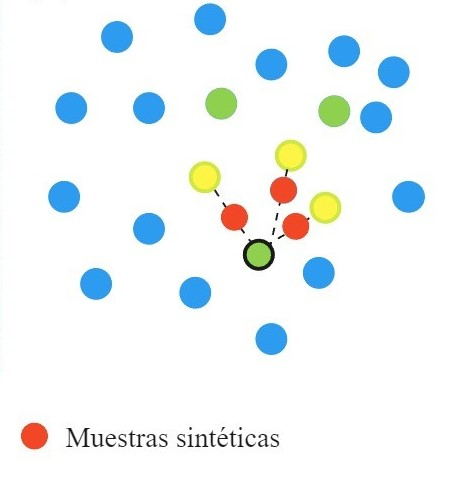
\includegraphics[height=5cm]{./Figures/SMOTE_c.jpg}}
	\caption{Representación esquematica del algoritmo SMOTE\protect\footnotemark.}\label{fig:SMOTEc}
	   \label{fig:SMOTE}
\end{figure}

\footnotetext{Imagen adaptada de Schubach, Max; Re, Matteo; Robinson, Peter y Valentini, Giorgio. (2017). Imbalance-Aware Machine Learning for Predicting Rare and Common Disease-Associated Non-Coding Variants. Scientific Reports. 7. 10.1038/s41598-017-03011-5.}

En suma, SMOTE permite generar ejemplos sintéticos que sean relativamente cercanos en el espacio de 
características con respecto a las muestras existentes de la clase minoritaria. Además, las muestras 
pueden crearse en la cantidad que sea requerida. Por lo tanto, en escenarios donde el conjunto de 
datos no solo está desbalanceado sino que también presenta una escasez de muestras, la aplicación 
de SMOTE resulta particularmente efectiva \citep{CITE:37} \citep{CITE:38}.

%----------------------------------------------------------------------------------------
% 2.2.3 Métricas de evaluación en modelos de clasificación
\subsection{Evaluación de modelos de clasificación}
Para evaluar el desempeño de un modelo de clasificación binaria se suele emplear una matriz de confusión. 
Esta matriz se ilustra en la figura \ref{fig:MatrizConfusion}, donde las columnas representan la clase 
predicha y las filas corresponden a las clases reales. 
A partir de esta tabla, se definen cuatro indicadores:

\begin{itemize}
	\item Verdaderos positivos (TP, por sus siglas en inglés): asignaciones positivas correctas.
	\item Verdaderos negativos (TN, por sus siglas en inglés): asignaciones negativas correctas.
\item Falsos positivos (FP, por sus siglas en inglés): asignaciones positivas incorrectas, es decir que
indican la presencia de una condición cuando la misma en realidad no está presente.
\item Falsos negativos (FN, por sus siglas en inglés): asignaciones negativas incorrectas, lo que significa
que indican la ausencia de una condición cuando en realidad está presente.
\end{itemize}

\begin{figure}[h!]
	\centering
	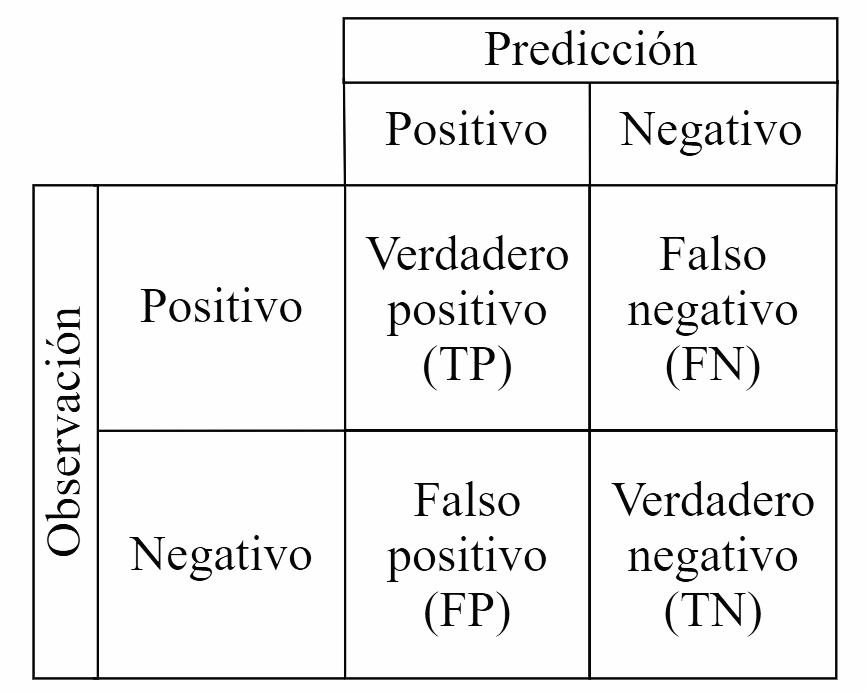
\includegraphics[width=0.5\textwidth]{./Figures/MatrizConfusion.jpg}
	\caption{Matriz de confusión.}\label{fig:MatrizConfusion}
\end{figure}

En el ámbito médico, el falso negativo puede ocasionar las consecuencias más graves para la salud del 
paciente. En este trabajo en particular, implica el riesgo de no tomar las medidas necesarias para un 
tratamiento adecuado, lo cual puede incurrir en que el paciente experimente un evento cardiovascular 
adverso mayor. En consecuencia, es de gran importancia minimizar la tasa de falsos negativos al máximo, 
aún si esto implica un aumento de falsos positivos. Si bien este incremento puede implicar la necesidad de 
destinar más recursos médicos para realizar pruebas adicionales o tratamientos innecesarios, se garantiza 
que menos casos sean pasados por alto \citep{CITE:40}.

A partir de los valores de TP, TN, FP y FN se definen diferentes métricas para evaluar el desempeño de 
un modelo de clasificación. A continuación, se explican algunas en detalle.

\subsubsection{\emph{Precision}}
La presición o \emph{precision} es una métrica que permite conocer la proporción de ejemplos clasificados 
correctamente como positivos sobre el total de ejemplos clasificados como positivos. Una alta precisión 
indica que el modelo tiene una baja tasa de falsos positivos y clasifica correctamente la mayoría de las 
instancias positivas. La expresión matemática que describe este comportamiento es la siguiente:

\begin{equation}
	\label{eq:precision}
	Precision = \frac{TP}{TP + FP}
\end{equation}


\subsubsection{\emph{Recall}}
La sensibilidad, \emph{recall} o tasa positiva real (TPR) es una métrica que mide la proporción de ejemplos 
clasificados correctamente como positivos en relación con el total de ejemplos positivos. Por lo tanto, se 
mide la capacidad de identificar la mayoría de las muestras positivas presentes. La siguiente ecuación 
matemática describe este comportamiento:

\begin{equation}
	\label{eq:recall}
	Recall = \frac{TP}{TP + FN}
\end{equation}


\subsubsection{\emph{F1-Score}}
La métrica \emph{F1-Score} es la media armónica entre \emph{precision} y \emph{recall}. Dado que tiene 
en cuenta tanto a los FP cómo los FN, se emplea para evaluar un modelo cuando el conjunto de datos es 
desequilibrado. La fórmula matemática que describe este comportamiento es la siguiente:

\begin{equation}
	\label{eq:f1score}
	F1\,score = \frac{2}{\nicefrac{1}{Precision} + \nicefrac{1}{Recall}} = 2\cdot\frac{Recall \cdot Precision}{Recall + Precision}
\end{equation}

\subsubsection{\emph{Accuracy}}
La exactitud o \emph{accuracy} es una métrica que mide la proporción de muestras clasificadas correctamente 
sobre el total de muestras evaluadas y se describe matemáticamente como:

\begin{equation}
	\label{eq:accuracy}
	Accuracy = \frac{TP + TN}{TP + TN + FP + FN}
\end{equation}

\subsubsection{\emph{Specificity}}
La especificidad, \emph{specificity} o tasa negativa real (TNR) se define como la proporción de falsos positivos 
sobre el total de negativos reales. Es una métrica exactamente opuesta a la sensibilidad y esta dada por:

\begin{equation}
	\label{eq:specificity}
	Specificity = \frac{TN}{TN + FP}
\end{equation}


\subsubsection{Curva ROC y AUC}
La curva ROC es una representación gráfica que muestra la tasa de verdaderos positivos (sensibilidad)
en función de la tasa de falsos positivos (1 - especificidad) a medida que se varía el umbral de 
clasificación. Si bien puede ser de utilidad visualizar la curva ROC, en muchas casos la información 
puede resumirse en la métrica AUC (acrónimo de \emph{Area Under the Curve}), que mide el área bajo la curva 
ROC. En general, cuanto más alto sea el AUC, mejor es el desempeño del clasificador. 

En la figura \ref{fig:ROC_a}, se puede observar un clasificador ideal en el cual las curvas de TP y TN no se 
superponen en absoluto, lo que resulta en un AUC igual a 1. Por el contrario, en la figura \ref{fig:ROC_c}, 
se muestra un clasificador de predicción aleatoria, donde la curva ROC es una línea recta con una pendiente unitaria. 
En este caso, las curvas de TP y TN se superponen por completo, lo que da como resultado un AUC de 0.5. 
En la figura \ref{fig:ROC_b}, se observa un caso intermedio en el que hay cierta superposición entre las curvas 
de TP y TN. En general, la mayoría de los modelos de clasificación binaria tienen un AUC entre 0.5 y 1. Es poco 
común encontrar un clasificador con un AUC menor que 0.5, ya que esto indicaría que las predicciones están invertidas.

\begin{figure}[h!]
	\centering
	\subcaptionbox{Clasificador perfecto.\label{fig:ROC_a}}%
  	[0.3\linewidth]{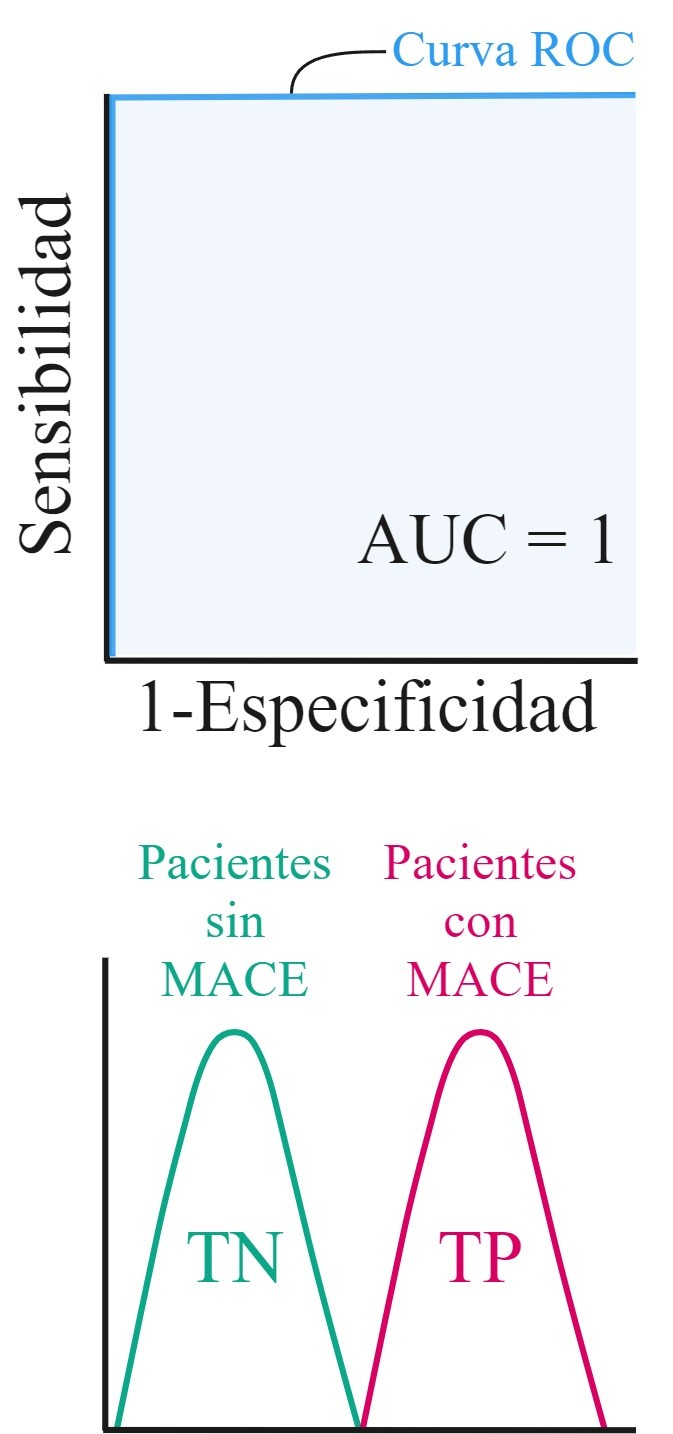
\includegraphics[height=10cm]{./Figures/ROC_a.jpg}}
	\hspace{1em}
	\subcaptionbox{Clasificador con buen \\poder predictivo.\label{fig:ROC_b}}
	[0.3\linewidth]{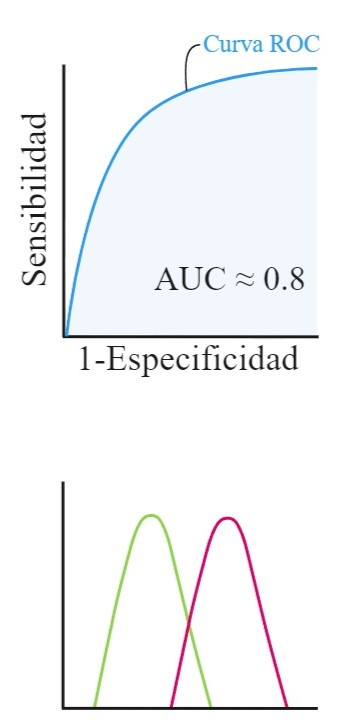
\includegraphics[height=10cm]{./Figures/ROC_b.jpg}}
	\hspace{1em}
	\subcaptionbox{Clasificador sin poder predictivo.\label{fig:ROC_c}}
	[0.3\linewidth]{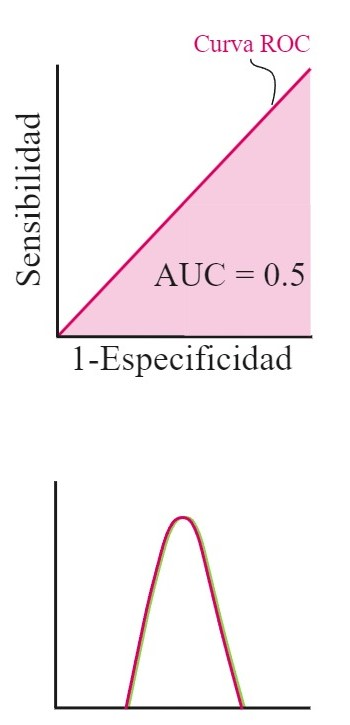
\includegraphics[height=10cm]{./Figures/ROC_c.jpg}}
	\caption{Representación gráfica de la curva ROC y las distribuciones de TP y TN\protect\footnotemark.}
\end{figure}
\footnotetext{Imagen adaptada de Glen, S. (2019). ROC Curve Explained in One Picture. Data Science Central. https://www.datasciencecentral.com/roc-curve-explained-in-one-picture/}

Para el presente trabajo, se evaluaron todas las métricas mencionadas anteriormente. Sin embargo, se seleccionó 
el AUC como la métrica principal para medir el desempeño de los modelos. Esto se debe a que en el ámbito clínico 
resulta de gran relevancia analizar la relación de compromiso entre la sensibilidad y especificidad. En definitiva, 
se buscó encontrar un equilibrio óptimo entre la detección temprana de casos de MACE positivos (alta sensibilidad) 
y la minimización de falsas alarmas (alta especificidad). 


%----------------------------------------------------------------------------------------
%	2.3 PERCEPTRÓN MULTICAPA
%----------------------------------------------------------------------------------------
\section{Perceptrón multicapa}
\label{sec:Perceptrón multicapa}

Las redes neuronales artificiales (RNA), propuestas inicialmente por McCulloch y Pitts en 1943 
\citep{CITE:41}, son modelos computacionales que se inspiran en el funcionamiento del cerebro 
humano. Si bien existen diversos tipos de RNA, esta sección se centra en los perceptrones 
multicapa, puesto que es la red empleada en este trabajo. En particular, se se abordan diversos 
aspectos teóricos clave, como la arquitectura, el algoritmo de entrenamiento, la validación del 
modelo, los hiperparámetros y los optimizadores. 
%----------------------------------------------------------------------------------------
% 2.3.1 Perceptrón
\subsection{Perceptrón}
Un perceptrón, también conocido como neurona artificial o nodo, es el bloque fundamental de las 
RNA y fue propuesto por Frank Rosenblatt en 1957 \citep{CITE:43}. En la figura \ref{fig:Perceptron} se puede observar 
cómo un perceptrón recibe $n$ señales de entrada $X = (x_1, x_2, …, x_n)$, las cuales se multiplican 
por un peso $W = (w_1, w_2, …, w_n)$. Este comportamiento es análogo a la manera en que los 
pesos sinápticos influyen en las neuronas biológicas, ya que algunas entradas tienen mayor relevancia 
que otras. Por este motivo, las entradas se combinan como una suma ponderada por sus pesos 
($\sum_{i=1}^{n} W_i \cdot X_i$) y se suma un término independiente conocido como \emph{bias} o 
sesgo, que le otorga flexibilidad al perceptrón en la modelización de patrones complejos. 
Posteriormente, se aplica una transformación no lineal mediante una función de activación $g$, 
la cual determina la salida $\hat{y} $ del perceptrón \citep{CITE:35} \citep{CITE:42}. 
La descripción matemática de este comportamiento se expresa de la siguiente manera: 

\begin{equation}\label{eq:perceptron}
\begin{split}
	&\hat{y} = g(z) = g( \sum_{i=1}^{n} W^T \cdot X + b) \\
				&\hat{y} = g(x_1 \cdot w_1 + x_1 \cdot w_1 + … + x_n \cdot w_n + b)
\end{split}
\end{equation}

\begin{figure}[h!]
	\centering
	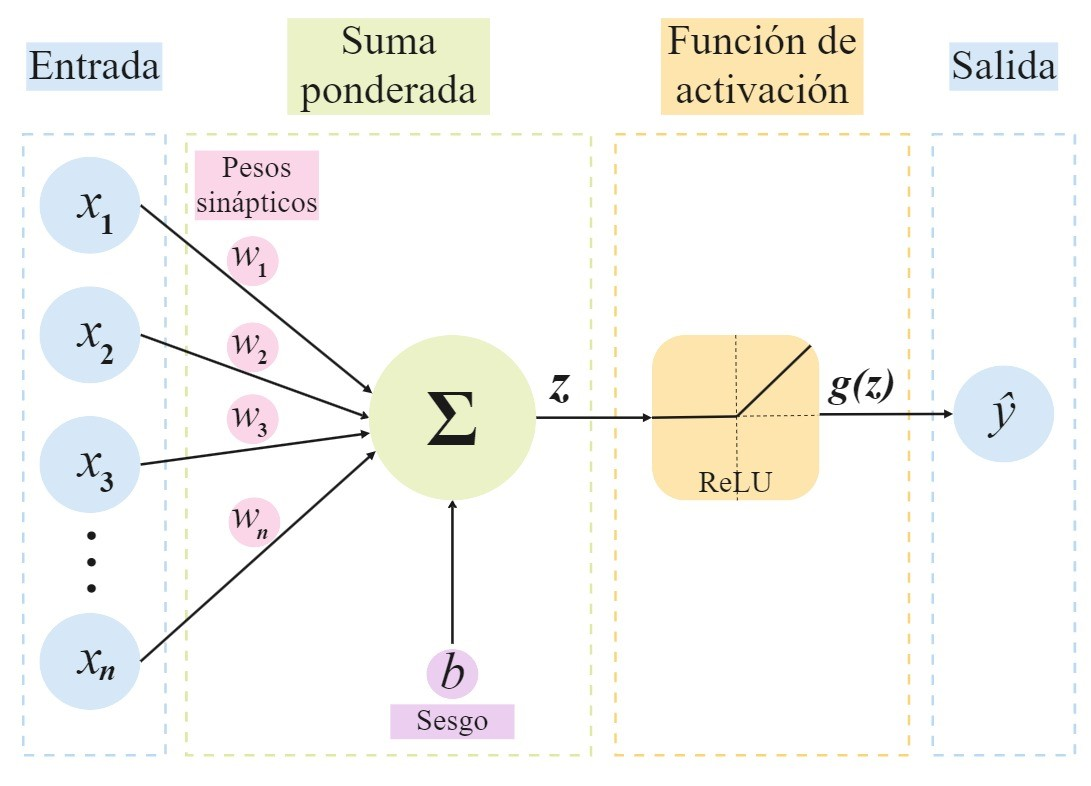
\includegraphics[width=\textwidth]{./Figures/Perceptron.jpg}
	\caption{Representación de un perceptrón.}
	\label{fig:Perceptron}
\end{figure}


%----------------------------------------------------------------------------------------
% 2.3.2 Arquitectura del perceptrón multicapa
\subsection{Arquitectura del perceptrón multicapa}

Un perceptrón multicapa (MLP, por sus siglas en inglés), también conocido como \emph{feedforward neural network} es 
una arquitectura de RNA ampliamente utilizada en el campo del aprendizaje profundo. Como se aprecia en la figura \ref{fig:MLP}, 
un MLP está compuesto por tres capas: capa de entrada o \emph{input layer}, capa oculta 
o \emph{hidden layer} y capa de salida o \emph{output layer}. 
A su vez, cada capa está formada por neuronas artificiales. La arquitectura del MLP es conocida como \emph{feedforward} 
puesto que la información siempre fluye desde la capa de entrada hacia la capa de salida a través de las capas ocultas, 
sin conexiones de retroalimentación. Cuando una RNA tiene dos o más capas ocultas, se lo conoce como una red neuronal 
profunda o \emph{deep neural network} (DNN) \citep{CITE:35} \citep{CITE:44}. 

\begin{figure}[h!]
	\centering
	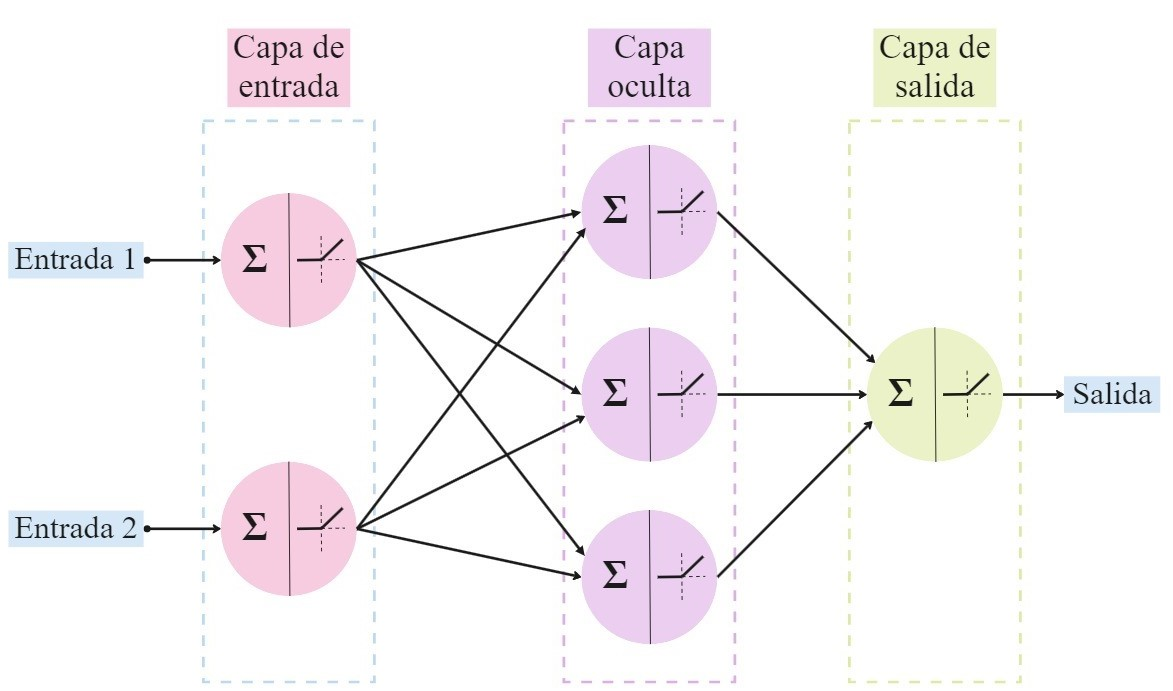
\includegraphics[width=\textwidth]{./Figures/MLP.jpg}
	\caption{Representación de un perceptrón multicapa \\ \emph{fully connected}.}
	\label{fig:MLP}
\end{figure}

Como se aprecia en la figura \ref{fig:MLP}, todos los nodos de una capa se encuentran conectados con todos los nodos de las 
capas adyacentes. El número de neuronas en la capa de entrada está definido por la cantidad de variables independientes 
del modelo, mientras que el número de nodos de la salida es la cantidad de variables dependientes. Además, el número de 
capas ocultas y su cantidad de neuronas dependen de la complejidad del modelo en cuestión, y son parámetros importantes 
a tener en cuenta durante el desarrollo del mismo \citep{CITE:42}.

La configuración del perceptrón multicapa de la figura \ref{fig:MLP} se conoce como \emph{fully connected}, ya que todos 
los nodos de una capa están conectados con todos los nodos de las capas adyacentes. Sin embargo, existen otros tipos de 
capas con diferentes estructuras de conexión. Por ejemplo, las capas de abandono o \emph{dropout} introducen la omisión de 
algunos nodos durante el entrenamiento de forma aleatoria para reducir el sobreajuste \citep{CITE:44} \citep{CITE:45}.



%----------------------------------------------------------------------------------------
% 2.3.3 Algoritmo de entrenamiento
\subsection{Algoritmo de entrenamiento}

\subsubsection{Forward propagation}
\subsubsection{Backpropagation}

%----------------------------------------------------------------------------------------
% 2.3.4 Validación del modelo
\subsection{Validación del modelo}

%----------------------------------------------------------------------------------------
% 2.3.5 Optimización del modelo
\subsection{Optimización del modelo}

%----------------------------------------------------------------------------------------
% 2.3.6 Hiperparámetros del modelo
\subsection{Hiperparámetros del modelo}

